\section{Empirical Observations: The Moving Learning Edge}
\label{sec:obs-preliminary}
This section dissects the training dynamics of GRPO-style RLVR to identify what makes a 
prompt useful for policy optimization and why effective selection in RLVR is an online tracking problem. 
We first recall why low-utility prompts produce no GRPO learning signal, then show that the useful 
prompts concentrate at a moving edge characterized by intermediate difficulty and high uncertainty. {The experimental details are reported in Appendix~\ref{sec:preliminary-setup}.}

% \red{The detailed experimental setting is described in Appendix~\ref{appendix:preliminary-experiment-setting}}.
% \red{till here}
% \begin{figure}[t]
%     \centering
%     % Four independent panels, each generated by its own Python script
%     % under unified style (see ICML2026-submission-figure-script-drawio-todo/wandb-figure/).
%     \begin{minipage}[t]{0.245\linewidth}
%         \centering
%         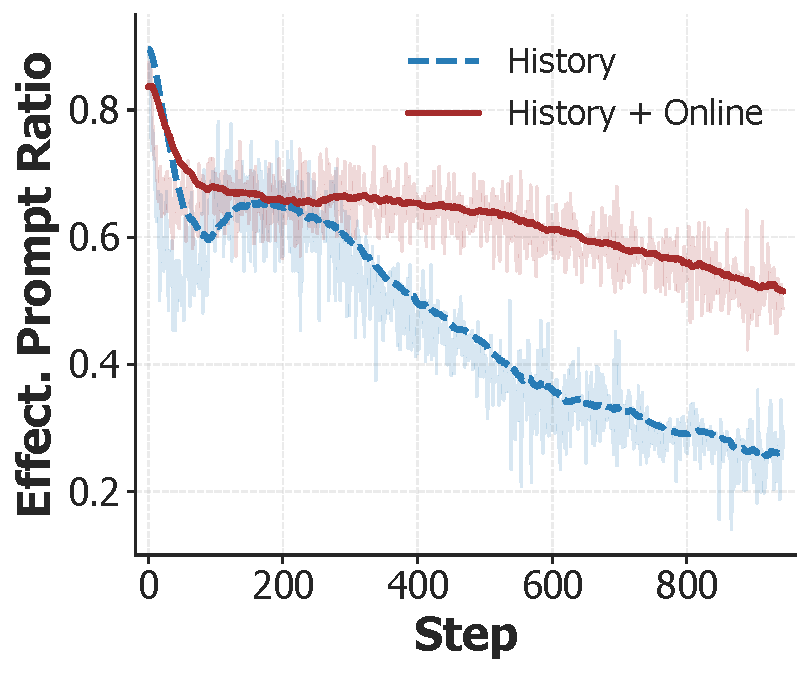
\includegraphics[width=\linewidth]{figures/intro/intro_a_eff_ratio.pdf}
%         \\[-2pt]{\footnotesize\textbf{(a)}\par}
%     \end{minipage}\hfill
%     \begin{minipage}[t]{0.245\linewidth}
%         \centering
%         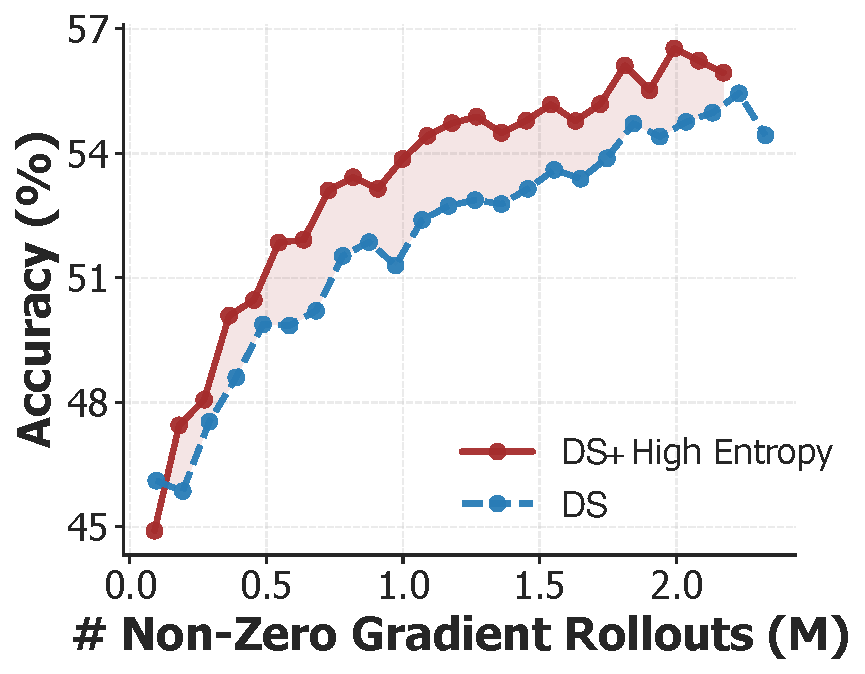
\includegraphics[width=\linewidth]{figures/intro/intro_b_high_entropy-backup.pdf}
%         \\[-2pt]{\footnotesize\textbf{(b)}\par}
%     \end{minipage}\hfill
%     \begin{minipage}[t]{0.245\linewidth}
%         \centering
%         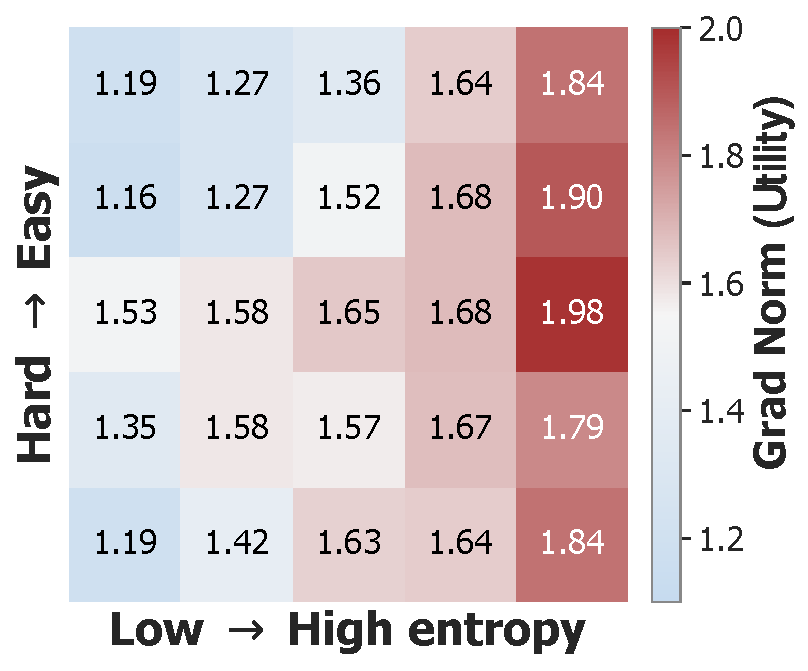
\includegraphics[width=\linewidth]{figures/intro/intro_c_heatmap-backup.pdf}
%         \\[-2pt]{\footnotesize\textbf{(c)}\par}
%     \end{minipage}\hfill
%     \begin{minipage}[t]{0.245\linewidth}
%         \centering
%         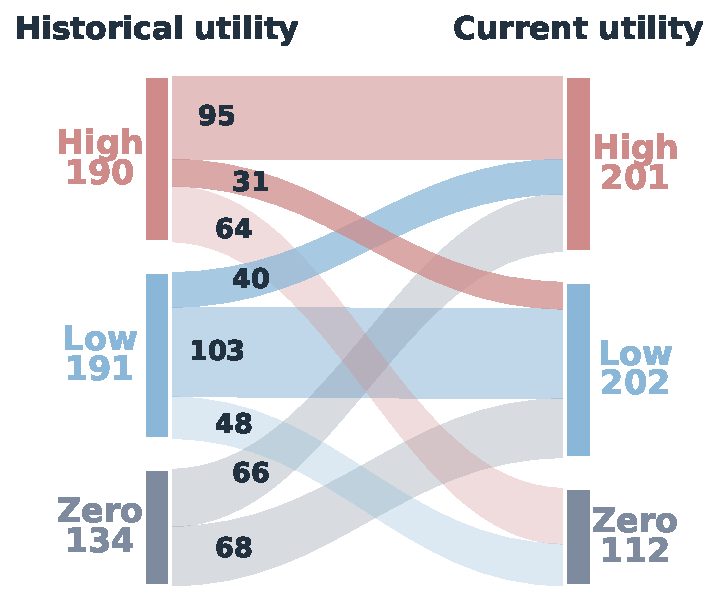
\includegraphics[width=\linewidth]{figures/intro/intro_d_sankey.pdf}
%         \\[-2pt]{\footnotesize\textbf{(d)}\par}
%     \end{minipage}
%     \caption{\textbf{Four empirical observations motivating HIVE.}
%     (a) Selection only based on historical statistics becomes increasingly stale during training, while online verification retains more effective prompts.
%     (b) Among prompts with non-zero gradients, prioritizing high-entropy
%         prompts improves accuracy at the same rollout budget.
%     (c) Gradient utility concentrates at an intermediate-difficulty,
%         high-entropy learning edge.
%     (d) Across two checkpoints (steps 500 and 1000), a large fraction of sampled
%         prompts shift between High, Low, and Zero utility classes, so
%         prompts selected by historical metadata no longer match the
%         current policy's utility distribution. \red{(1) need to re-write the corresponding prelimiary analysis and (2) revise the reference of these four subfigures.}
%     }
%     \label{fig:intro-a-b}
%     \vskip -0.15in
% \end{figure}
\begin{figure}[t]
    \centering
    \captionsetup[subfigure]{labelformat=parens,labelsep=none,font=footnotesize,justification=centering}
    % Four independent panels, each generated by its own Python script
    % under unified style (see ICML2026-submission-figure-script-drawio-todo/wandb-figure/).
    \begin{subfigure}[t]{0.241\linewidth}
        \centering
        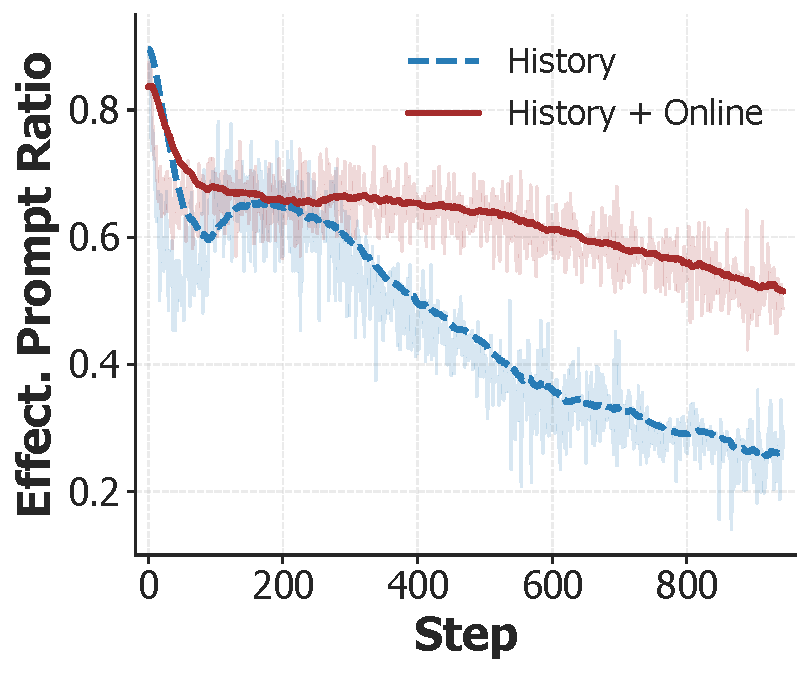
\includegraphics[width=\linewidth]{figures/intro/intro_a_eff_ratio.pdf}
        \vspace{-6pt}
        \caption{}
        \label{fig:intro-history-staleness}
    \end{subfigure}\hfill
    \begin{subfigure}[t]{0.245\linewidth}
        \centering
        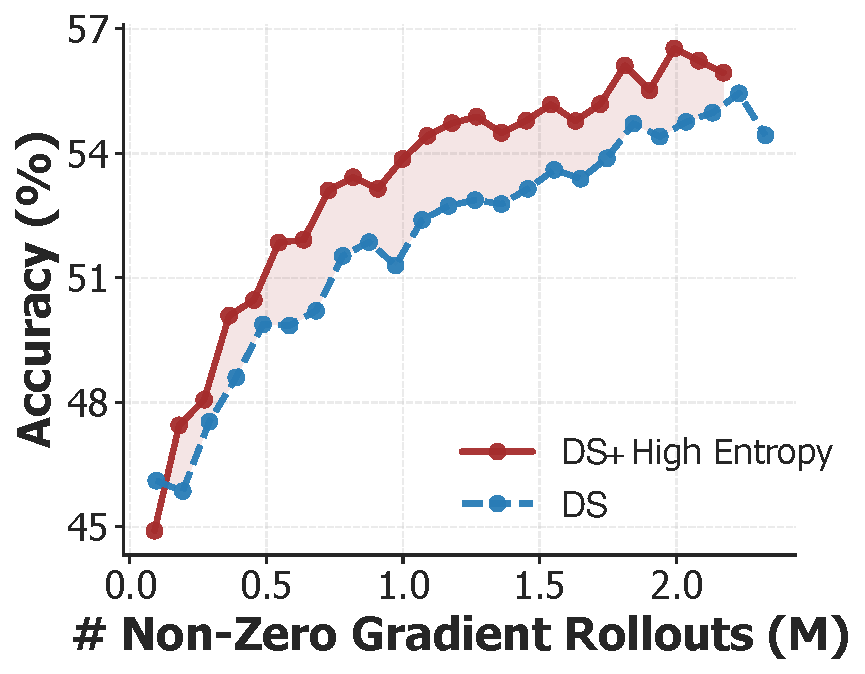
\includegraphics[width=\linewidth]{figures/intro/intro_b_high_entropy-backup.pdf}
        \vspace{-6pt}
        \caption{}
        \label{fig:intro-high-entropy}
    \end{subfigure}\hfill
    \begin{subfigure}[t]{0.245\linewidth}
        \centering
        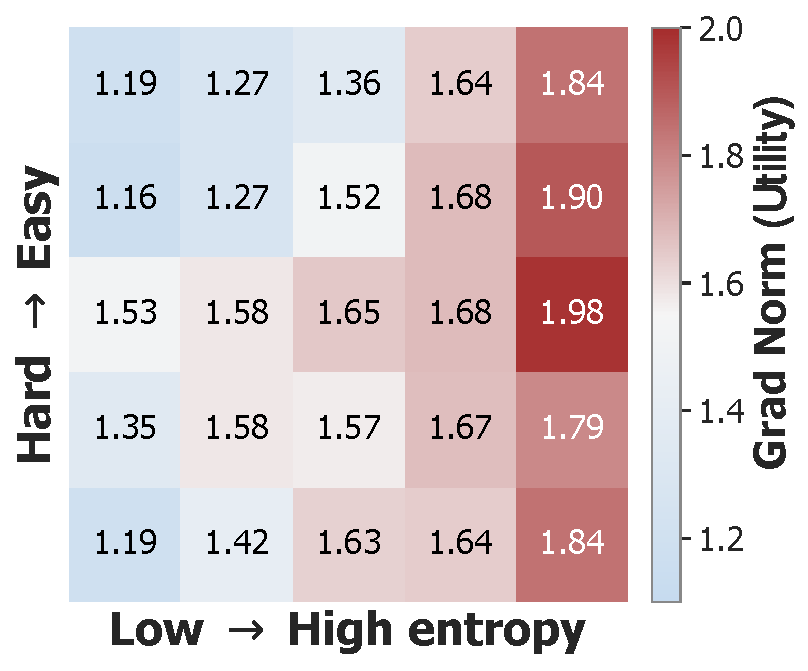
\includegraphics[width=\linewidth]{figures/intro/intro_c_heatmap-backup.pdf}
        \vspace{-6pt}
        \caption{}
        \label{fig:intro-learning-edge}
    \end{subfigure}\hfill
    \begin{subfigure}[t]{0.241\linewidth}
        \centering
        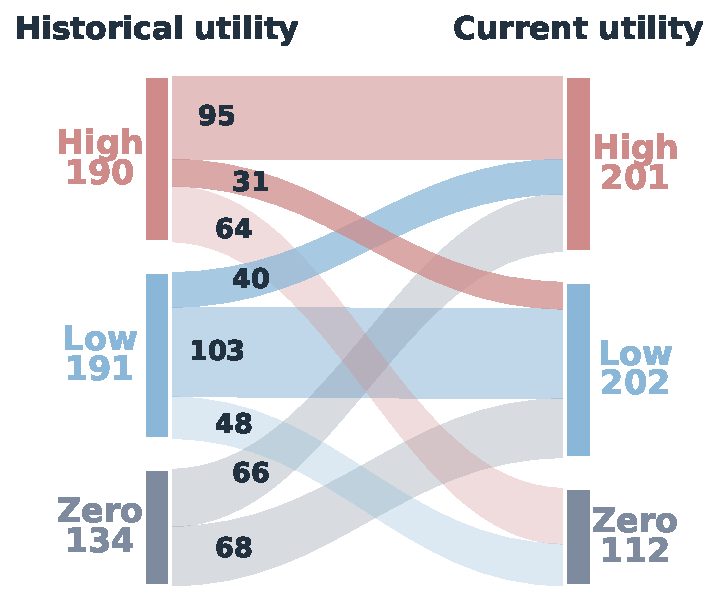
\includegraphics[width=\linewidth]{figures/intro/intro_d_sankey.pdf}
        \vspace{-6pt}
        \caption{}
        \label{fig:intro-utility-shift}
    \end{subfigure}
    \caption{\textbf{Empirical observations.}
    (a) Selection only based on historical statistics becomes increasingly stale during training, while online verification retains more effective prompts.
    (b) Among prompts with non-zero gradients, prioritizing high-entropy
        prompts improves accuracy at the same rollout budget.
    (c) Gradient utility concentrates at an intermediate-difficulty,
        high-entropy learning edge.
    (d) Across two checkpoints (steps 500 and 1000), a large fraction of sampled
        prompts shift between High, Low, and Zero utility classes, so
        prompts selected by historical metadata no longer match the
        current policy's utility distribution.
    }
    \label{fig:intro-a-b}
    \vskip -0.15in
\end{figure}

\begin{figure}[t]
    \centering
    % \includegraphics[width=1.0\linewidth]{figures/icml2026-framework-7.png}
    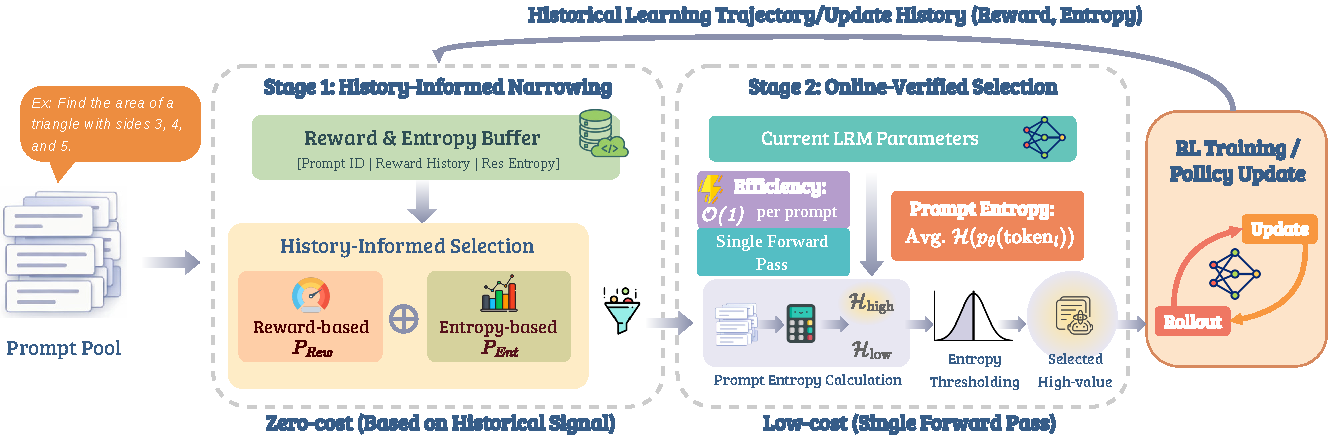
\includegraphics[width=1.0\linewidth]{figures/icml2026-framework-8-compressed.pdf}
    \caption{Overview of HIVE. \textbf{HIVE tracks the moving learning edge by decomposing prompt selection into two stages.}
    \textbf{Stage 1} uses historical reward trajectories and response-side entropy for efficient coarse narrowing. \textbf{Stage 2} computes prompt-side entropy under the current policy for low-cost online verification, rejecting stale candidates before rollout.}
    \label{fig:framework}
    \vskip -0.2in
\end{figure}


\textbf{Zero-variance prompts produce vanishing advantages.}
Group relative policy optimization (GRPO)~\cite{shao2024deepseekmath} is widely used in RLVR for reasoning models~\cite{guo2025deepseek,yang2025qwen3technicalreport}. For a prompt $q$, GRPO samples a group of responses $\{o_i\}_{i=1}^G$ and optimizes
% \begin{equation}
% \label{eq:grpo}
% \begin{aligned}
% \mathcal{J}_{\mathrm{GRPO}}(\theta)
% =
% \mathbb{E}_{\substack{
% q \sim P(Q), \{o_i\}_{i=1}^G \sim \pi_{\theta_{\mathrm{old}}}(\cdot \mid q)
% }}
% \Bigg[
% \frac{1}{G}\sum_{i=1}^G \frac{1}{|o_i|}
% \sum_{t=1}^{|o_i|} \Bigg(
% \min \left(\rho_{i,t}(\theta) \hat{A}_{i, t},&\\
%  \operatorname{clip}(\rho_{i,t}, 1 \pm \varepsilon) \hat{A}_{i, t}\right)
% - \beta D_{\mathrm{KL}}(\pi_\theta \,\|\, \pi_{\mathrm{ref}})
% \Bigg)
% \Bigg].&
% \end{aligned}
% \end{equation}
\begin{equation}
\label{eq:grpo}
\begin{aligned}
\mathcal{J}_{\mathrm{GRPO}}(\theta)
&=
\mathbb{E}_{\substack{
q \sim P(Q),\ \{o_i\}_{i=1}^{G} \sim \pi_{\theta_{\mathrm{old}}}(\cdot \mid q)
}}
\Biggl\{
\frac{1}{G}\sum_{i=1}^{G}\frac{1}{|o_i|}
\sum_{t=1}^{|o_i|}
\biggl(
\min \Bigl[
\frac{\pi_{\theta}(o_{i,t}\mid q,o_{i,<t})}{\pi_{\theta_{\mathrm{old}}}(o_{i,t}\mid q,o_{i,<t})}\hat{A}_{i,t}, \\
&\qquad\qquad\;
\operatorname{clip}(
\frac{\pi_{\theta}(o_{i,t}\mid q,o_{i,<t})}{\pi_{\theta_{\mathrm{old}}}(o_{i,t}\mid q,o_{i,<t})}, 1-\varepsilon, 1+\varepsilon
)\hat{A}_{i,t}
\Bigr]
-\beta D_{\mathrm{KL}}\!\left[
\pi_{\theta}\,\|\,\pi_{\mathrm{ref}}
\right]
\biggr)
\Biggr\},
\end{aligned}
\end{equation}
% where
% \begin{equation}
%     \mathcal{L}^{\mathrm{clip}}_{i,t}(\theta)=\min \left(\rho_{i,t}(\theta) \hat{A}_{i, t}, \operatorname{clip}(\rho_{i,t}, 1 \pm \varepsilon) \hat{A}_{i, t}\right).
% \end{equation}
% where the group-normalized advantage $\hat{A}_{i}$ is computed as follows\red{ need more justifications on the notations}:
where $P(Q)$ is the prompt distribution, $G$ is the response group size, and $o_{i,t}$ denotes the $t$-th token
of response $o_i$. The KL penalty with weight $\beta$ anchors $\pi_\theta$ to the
reference policy $\pi_{\mathrm{ref}}$. Since RLVR gives a sequence-level reward $r_i$, all tokens in $o_i$
share the group-normalized advantage $\hat{A}_{i,t}=\hat{A}_{i}$:
\begin{equation}
\label{eq:grpo_advantage}
\hat{A}_{i} = \frac{r_i - \mathrm{mean}(\{r_i\}_{i=1}^G)}{\mathrm{std}(\{r_i\}_{i=1}^G)}.
\end{equation}
When all sampled responses for a prompt receive the same reward, the reward variance is zero and the prompt contributes no informative policy-gradient signal. Such prompts are either already easy for the current policy or still too hard to discriminate among sampled responses. Rollout scaling therefore wastes compute unless it avoids these zero-variance regions.

\textbf{Utility concentrates at an intermediate-difficulty, high-entropy edge.}
Zero-variance filtering is necessary but not sufficient: among prompts with non-zero gradients, some still provide much stronger learning signal than others. Following previous analyses~\cite{kim2025mitigatinglengthbiasrlhf,paul2021DataDiet,fayyaz2022bertdatadietfinding,singhal2024aCOLM}, we use length-normalized gradient norm as a proxy for per-prompt utility and study how it varies with empirical difficulty and response-side entropy.

Figure~\ref{fig:intro-learning-edge} shows two consistent patterns. First, within a fixed difficulty band, gradient norm increases with response-side entropy. Second, at a fixed entropy level, utility follows an inverted-U shape over 
difficulty: trivial prompts and intractable prompts have low utility, while intermediate-difficulty prompts have 
higher utility. The strongest learning signal appears at the intersection of these two conditions. We call this 
region the \textit{learning edge}. This observation explains why merely removing zero-variance prompts is too 
coarse: \textit{the best rollout budget should be allocated to prompts that are both learnable and uncertain under the 
current policy}.

\textbf{Historical metadata becomes stale as the edge moves.}
As the policy updates, the model's state of knowledge changes, and historical 
metadata such as reward trajectories and response entropies can quickly become stale~\cite{cui2025entropymechanismreinforcementlearning,tomihari2026learningdynamicsrlposttraining,li2026stalefeedbackcoevolvingcritics}. 
To quantify this effect, we compare prompts selected by historical metadata from the previous training window 
with prompts selected by online metrics recomputed under the current policy. As shown in Figure~\ref{fig:intro-utility-shift}, 
historical selection yields lower current gradient norms, whereas online selection isolates prompts with high utility. Figure~\ref{fig:intro-utility-shift} further shows that prompts frequently move among High, Low, and Zero utility classes across training steps. Together, these results indicate that: \textit{a selector must revalidate candidate prompts under the current policy to keep tracking the moving edge}.
